\documentclass[12pt]{article}
\usepackage{amsmath}
\usepackage{emptypage}
\usepackage{blindtext}
\usepackage{titlesec}
\usepackage[hidelinks]{hyperref}
\usepackage{graphicx}
\usepackage[italian]{babel}
\graphicspath{ {./images/} }
\author{}
\title{
    \huge 
        \textbf{Università degli Studi di Modena e Reggio Emilia}
    \large
        \par Dipartimento di Scienze Fisiche, Informatiche e Matematiche
        \par Corso di laurea in Informatica
    \vfil
        \huge \par \textbf{Engim report service}
    \vfil
    \normalsize
    \begin{tabular}{lp{0.4\textwidth}l}
      Relatore: & & Candidato: \\
      Prof. Claudia Canali & &  Dumitru Frunza \\
      \end{tabular}
}
\date{Anno academico 2021/2022}
\linespread{1.5}



\begin{document}
\maketitle
\thispagestyle{empty}
\newpage 
\thispagestyle{empty}
\
\newpage
\pagenumbering{roman}
\addtocounter{page}{0}
\listoffigures
\newpage
\phantomsection
\tableofcontents
\addcontentsline{tesi}{Infrastruttura}{Infrastruttura}
\newpage

\pagenumbering{arabic}
\addtocounter{page}{0}
\section{Introduzione}
\section{Engim Srl}
\subsection{L'azienda}
Engim è una società che si occupa di creare soluzioni tecnologiche in ambito 
ICT, telecomunicazioni, sistemi di gestione e mobilità. Da oltre 10 anni operano 
nel mercato della tracciabilità di flotte e attività e della 
sicurezza dei lavoratori in solitario.
\\ ServizioGPS è il noleggio di tracker gps per veicoli lavoratori. 
Una prevalente parte dei clienti sono comuni che, tramite i prodotti Engim, 
tracciano il percorso delle macchine spazzaneve e spargisale.
I tracker possono essere prodotti fisici oppure un app per smartphone. A loro 
volta i prodotti fisici si dividono in fissi e mobili. Il servizio include
anche un gestionale per poter visualizzare, modificare o archiviare i propri dati.
\\ Twicetouch è noleggio di dispositivi di sicurezza individuale.
Il prodotto tutela i lavoratori in solitario mandando una segnalazione in caso di
emergenza. Esistono due tipi di rilevazione: 
\begin{itemize}
  \item caduta: l'accelerometro del dispositivo rileva un urto pericoloso
  \item assenza di movimento: il lavoratore non si è mosso per un lasso prolungato di tempo, 
  quindi si presume che possa essere incosciente
\end{itemize}
Similmente a servizioGPS è possibile noleggiare un dispositivo fisico (badge) oppure
l'app per android. In entrambi i casi è possibile impostare i numeri in caso di 
emergenza, che riceveranno una chiamata e un messagio SMS.

\subsection{Infrastruttura}
Le tecnologie usate per servizioGPS sono le seguenti:
\begin{itemize}
  \item Ruby on rails full stack
  \item Mariadb e Redis come database
  \item Python come back end di supporto
  \item Java per il prodotti app 
\end{itemize}
\begin{figure}[h]
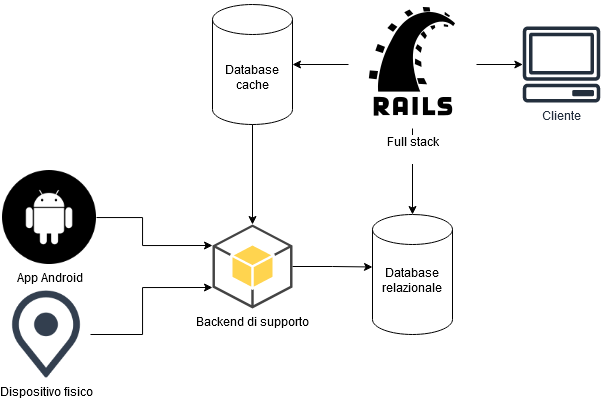
\includegraphics[scale = 0.6]{infrastructure.png}
\caption{Architettura}
\label{fig:mesh1}
\end{figure}
Ruby on Rails è usato per front-end e gran parte del backend di servizioGPS. 
Il fetcher invece si dedica esclusivamente alla elaborazione di coordinate gps,
per poter alleviare il carico di lavoro da Rails.
Allo stesso scopo il servizio si appoggia su molteplici server.
Uno di questi server è Amazon Web Services, un servizio di cloud computing 
che oltre al noleggio di un server tradizionale rende possibile 
anche un architettura a microservizi. 

\subsection{Microservizi}
Un servizio è un processo che: esegue specifiche operazioni autonomamente, 
risponde a eventi oppure rimane in attesa di una richiesta. 
Nel caso in cui queste operazioni vengano svolte continuamente, il servizio è 
estremamente vantaggioso. Non è però necessario che il servizio sia sempre in 
esecuzione se viene usato in maniera discontinua o per brevi periodi di tempo. 
I microservizi coprono questo ruolo, hanno le stesse caratteristiche di un servizio
ma eseguono solo su richiesta. 
\\ L'ambiente di esecuzione è completamente gestito da AWS, l'unica requisito per 
creare un microservizio è caricare il proprio codice. In questo caso viene 
noleggiato il tempo di calcolo invece che una macchiana fisica o virtuale.
L'ambiente viene creato al momento della richiesta, esegue il codice e cessa di 
esistere. 
Quando il microservizio non è attivo non ci sono costi.
\\ È bene tenere in mente due importanti caratteristiche dei microservizi:
\begin{itemize}
  \item L'ambiente non ha spazio di archiviazione, qualora sia necessario 
  salvare un file, bisogna caricarlo in un servizio di clound computing come S3
  \item Le tecnologie devono essere compatibili con l'infrastruttura sottostante,
  il che limita le nostre scelte
\end{itemize}
Avendo in mente queste considerazioni, un caso d'uso adatto ai microservizi 
è un servizio API che viene usato in maniera occasionale oppure per brevi periodi 
fissi.

\subsection{Sistema automatico di generazione di report}
Engim esegue una manutenzione annuale di database, che consiste nell'archiviazione
dei dati. Questi possono essere salvati dal cliente, nel caso fosse interessato 
o necessitato, sotto forma di pdf oppure xls.
\\ 
Le informazioni più importanti sono l'elenco e le specifiche di tutte le "attività". 
Un'attività contiente una serie di dati, tra cui: coordinate
gps, costi di lavoro, tempo di lavoro e altro.  
Al momento il servizio è implementato da Rails tramite una gemma di ruby. 
Il sistema attuale crea un istanza di chrome, l'istanza contiene un HTML
che si desidera convertire in pdf e infine avviene il parsing del documento.
\\ Questo ha una serie di gravi problemi:
\begin{itemize}
  \item La necessità di avviare un istanza di Chrome e il parsing di un HTML è
  estremamente costoso dal punto di vista delle risorse
  \item Il parsing di un HTML è anche estremamente costoso in termini di tempo,
  aggravato dalle lunghe query dovute alla grande mole di dati 
  \item Il  parsing tende a essere poco affidabile
\end{itemize}
La natura del nostro problema rende molto facile la scelta di un microservizio.
L'operazione è ripetitiva, ben definita e usata per brevi periodi. Altri vantaggi 
importanti sono il risparmio di risorse del server, che evita di gravare sulle 
operazioni più critiche, e la possibilità di usare il microservizio per qualsiasi 
altro prodotto Engim.


\section{Requisiti del progetto}
\subsection{Descrizione}
Il progetto è una funzione lambda su AWS, ovvero un microservizio. La funzione 
è chiamata tramite https, e prende in input un json. Il json è contiene i dati 
di autenticazione e il contenuto da convertire in pdf. L'autenticazione avviene 
tramite token e whitelist, questi sono salvati come variabili di ambiente su AWS.
I contenuti invece sono divisi in sezioni per permettere facilitare la dinamicità 
della stampa.
\\ Nel caso in cui la stampa sia avvenuta correttamente la funzione ritorna 200 e 
il link al file su S3. Se l'input della chiamata risulta errato, la funzione ritorna 
400 e un messaggio che descrivere l'errore. Infine se avviene un errore di connessione 
al bucket S3, la funzione ritornerà un errore 500.    
\\ Il progetto deve permettere l'implementazione di stampe diverse da quelle di servizioGPS
e di altri file di output come kml e xls. 

\subsection{User stories}
\subsection{Scelte del linguaggio}
Le lambda su AWS hanno il supporto per i linguaggi più popolari del momento, in
particolare ho preso in considerazione python, javascript e ruby. La libreria
che faceva di più al mio caso era pdfKit di javascript, che è un port di pdfkit
libreria di php per scrivere pdf senza dover far parsing di altri file.
Ruby aveva più libreria con parsing intermedi e python aveva libreria non mantenute.


\section{Sviluppo}
\subsection{Workflow}
Il mio senior ha deciso di fare un implementazione a grossi step, ogni volta
facendo un piccolo pezzo per poi controllare che tutto funzioni correttamente.
Ogni issue è uno step e a ogni step il progetto viene testato sia manualmente su
aws tramite simulazioni di richiesta sia con test automatizzati tramite mocha.

\subsection{Creazione di un file e salvataggio su S3}
La lamda è una funzione assincrona che viene eseguita ogni volta che riceve una
chiamata https. Bisogna prima di tutto creare una connessione con il bucket di s3,
una volta creata questa connessione si può salvare un file passando il filepath
oppure uno stream di data e avremo salvato il file su S3

\subsection{Stampa di un file pdf da un json}
Le operazioni utili al mio scopo text per scrivere una stringa,
stroke per disegnare una linea e infine è possibile manipolare colori e font.
Inizialmente avevo deciso di programmare in maniera funzionale perché risultava
una logica più semplice essendo un breve script, con l'aumentare della complessità
e con il modo di esportare di javascript ho pensato che una classe fosse più adeguata.
Quindi c'è un costruttore che definisce la grandezza del documento, questo mantiene
la relazione di un foglio A4 (circa 1.41) in modo che stampa e visualizzazione sono
sempre molto comodi. Dopo l'inizializzazione si inizia la scrittura dei blocchi.
Ogni json potrebbe avere un header, body e table. Se uno dei 3 manca, non verrà
scritto e gli altri si organizzeranno di conseguenza. Ogni metodo di scrittura
controlla che non ci siano dati mancanti che possano nuocere alla stampa come ad
esempio se manca un titolo non è una stampa valida, e ritornano 400. Se tutto va
bene e la stampa va a buon fine, è possibile mandare l'oggetto con get document.
Ogni possibile caso è testato con mocha, la connessione con AWS è mochata tramite
aws-sdk e gran parte dei dati è generata casualmente tramite faker.
Se tutto va a buon fine il programma ritorna 200 e il link del download.

\section{Implementazione}
\section{Applicazione e performance}
\section{Conclusione}
\section{Appendici}
\section{Bibliografia}
\end{document}